\documentclass[11pt,a4paper]{article}
\usepackage[T1,T2A]{fontenc}
\usepackage[a4paper,letterpaper,top=20mm,bottom=15mm,nohead,nofoot,left=20mm,right=13mm]{geometry}
\usepackage[utf8]{inputenc}
\usepackage{cmap}
\usepackage[russian, english]{babel}
\usepackage{textcomp}
\usepackage{indentfirst}
\usepackage{rotating, graphicx}
\usepackage{mwe}
\usepackage{wrapfig}
\usepackage{hyperref}
\usepackage{caption}
\usepackage{multirow}
\usepackage{array}
\usepackage{makecell}
\usepackage{listings}
\usepackage{listingsutf8}

\lstset{
    frame=tb,
    extendedchars=false,
    inputencoding=utf8,
    numbers=left,
    language=Java,
    aboveskip=3mm,
    belowskip=3mm,
    showstringspaces=false,
    basicstyle=\normalsize\ttfamily,
    breaklines=true,
    breakatwhitespace=false,
    columns=fullflexible,
    tabsize=2,
    keepspaces=true,
    linewidth=\linewidth
}

\newcounter{imgcnt}
\setcounter{imgcnt}{1}

\begin{document}
\sloppy
\setlength{\footskip}{10mm}

\newpage\thispagestyle{plain}
\thispagestyle{empty}
\begin{center}
\textbf{МИНИСТЕРСТВО НАУКИ И ВЫСШЕГО ОБРАЗОВАНИЯ\\
РОССИЙСКОЙ ФЕДЕРАЦИИ\\[2ex]
\mbox{ФЕДЕРАЛЬНОЕ ГОСУДАРСТВЕННОЕ БЮДЖЕТНОЕ ОБРАЗОВАТЕЛЬНОЕ}\\
УЧРЕЖДЕНИЕ ВЫСШЕГО ОБРАЗОВАНИЯ\\
«ВЯТСКИЙ ГОСУДАРСТВЕННЫЙ УНИВЕРСИТЕТ»\\[2ex]
Институт математики и информационных систем\\[2ex]
Факультет автоматики и вычислительной техники\\[2ex]
Кафедра электронных вычислительных машин}
\end{center}
\vspace{40mm}

\begin{center}
Отчёт по лабораторной работе №3\\
по дисциплине\\[1ex]
<<Объектно-ориентированное \\программирование>>\\[1ex]
\end{center}
\vspace{54mm}
Выполнил студент гр. ИВТб-2302-05-00 \hspace{30mm} \rule[-0,5mm]{30mm}{0.15mm}\,/Матешко В.В./\\
\mbox{\tiny\hspace{112mm}(Подпись)}\\[2ex]
Проверил старший преподаватель \hspace{40mm} \rule[-0,5mm]{30mm}{0.15mm}\,/Шмакова Н.А/\\
\mbox{\tiny\hspace{112mm}(Подпись)}\\[2ex]
\vfill
\begin{center}
Киров\\
2026
\end{center}

\newpage
\topmargin = -35pt

\section*{\normalsize Цель работы}

Разработать веб-приложение, используя классы и особенности Java, демонстрирующее применение ООП и работу через Hibernate.

\section*{\normalsize Задание}

На основе предметной области разработать приложение на Java с веб-интерфейсом. Данные об объектах предметной области хранить в PostgreSQL. Для работы с БД использовать Hibernate, а для базовых CRUD-операций использовать \texttt{CrudRepository}.

\section*{\normalsize Требования к реализации}

\begin{enumerate}
    \item Использование языка программирования Java;
    \item Использование СУБД PostgreSQL;
    \item Использование сборщика Maven;
    \item Использование Hibernate для подключения к БД;
    \item \textbf{Требование к БД}: не менее 3-х связанных таблиц в 3-ей нормальной форме. Обязательно хотя бы одна связь не по наследованию;
    \item Веб-интерфейс;
\end{enumerate}

\newpage
\section*{\normalsize Ход работы}

\textbf{Предметная область:} универсальные API-подключения (VK и Telegram).

\subsection*{Описание классов предметной области}

\textbf{Базовый абстрактный класс \texttt{Api}:}
\begin{itemize}
    \item Тип класса и модификатор доступа: \texttt{public abstract class Api};
    \item Поля:
    \begin{itemize}
        \item \texttt{private Long id} --- первичный ключ;
        \item \texttt{protected String name} --- название API-подключения;
        \item \texttt{protected String baseUrl} --- базовый URL;
        \item \texttt{protected Organization organization} --- ссылка на организацию (many-to-one).
    \end{itemize}
    \item Методы:
    \begin{itemize}
        \item \texttt{public String initialize()} --- возвращает строку \texttt{"Initializing API..."};
        \item \texttt{public String fetchData(String command)} --- базовая реализация, возвращает строку \texttt{"Загрузка данных..."}; в потомках может переопределяться для предметной команды.
    \end{itemize}
    \item Конструкторы:
    \begin{itemize}
        \item \texttt{protected Api()} --- пустой конструктор для Hibernate;
        \item \texttt{protected Api(String name, String baseUrl)} --- инициализирует родительские поля \texttt{name} и \texttt{baseUrl}.
    \end{itemize}
    \item Геттеры/сеттеры:
    \begin{itemize}
        \item Для полей \texttt{id}, \texttt{name}, \texttt{baseUrl}, \texttt{organization} используются Lombok-аннотации \texttt{@Getter} и \texttt{@Setter}.
    \end{itemize}
\end{itemize}

\textbf{Класс \texttt{VkApi extends Api}:}
\begin{itemize}
    \item Тип класса и модификатор доступа: \texttt{public class VkApi extends Api};
    \item Поля:
    \begin{itemize}
        \item \texttt{private String version} --- версия VK API;
        \item \texttt{private String token} --- токен доступа;
        \item \texttt{private List<VkPost> posts} --- связанные посты (one-to-many).
    \end{itemize}
    \item Методы:
    \begin{itemize}
        \item \texttt{public String initialize()} --- наследует родительское поведение и может вызываться через API;
        \item \texttt{public String fetchData(String command)} --- обобщённый вызов команды для демонстрации полиморфного доступа;
        \item \texttt{public List<String> getText()} --- возвращает список текстов постов;
        \item \texttt{public List<Integer> getLike()} --- возвращает список значений лайков.
    \end{itemize}
    \item Конструкторы:
    \begin{itemize}
        \item \texttt{protected VkApi()} --- пустой конструктор для Hibernate;
        \item \texttt{public VkApi(String version, String token)} --- создаёт VK API с явными \texttt{version} и \texttt{token}, а \texttt{name/baseUrl} задаёт как \texttt{"VK"} и \texttt{"https://api.vk.com/method"};
        \item \texttt{public VkApi(String token)} --- создаёт VK API с токеном и версией по умолчанию \texttt{"5.199"}.
    \end{itemize}
    \item Геттеры/сеттеры:
    \begin{itemize}
        \item Для полей \texttt{version}, \texttt{token}, \texttt{posts} используются Lombok-аннотации \texttt{@Getter} и \texttt{@Setter}.
    \end{itemize}
\end{itemize}

\textbf{Класс \texttt{TgApi extends Api}:}
\begin{itemize}
    \item Тип класса и модификатор доступа: \texttt{public class TgApi extends Api};
    \item Поля:
    \begin{itemize}
        \item \texttt{private String botToken} --- токен бота;
        \item \texttt{private long chatId} --- идентификатор чата;
        \item \texttt{private List<TgPayload> payloads} --- связанные данные сообщений (one-to-many).
    \end{itemize}
    \item Методы:
    \begin{itemize}
        \item \texttt{public String initialize()} --- наследует родительское поведение и может вызываться через API;
        \item \texttt{public String fetchData(String command)} --- обобщённый вызов команды для демонстрации полиморфного доступа;
        \item \texttt{public List<String> sendMessage()} --- возвращает тестовые данные отправки сообщения;
        \item \texttt{public List<String> sendPhoto()} --- возвращает тестовые данные отправки фото.
    \end{itemize}
    \item Конструкторы:
    \begin{itemize}
        \item \texttt{protected TgApi()} --- пустой конструктор для Hibernate;
        \item \texttt{public TgApi(String botToken, long chatId)} --- создаёт Telegram API с токеном и чатом, а \texttt{name/baseUrl} задаёт как \texttt{"TG"} и \texttt{"https://api.telegram.org/bot"};
        \item \texttt{public TgApi(String botToken)} --- создаёт Telegram API только с токеном, \texttt{chatId} устанавливается в \texttt{0L}.
    \end{itemize}
    \item Геттеры/сеттеры:
    \begin{itemize}
        \item Для полей \texttt{botToken}, \texttt{chatId}, \texttt{payloads} используются Lombok-аннотации \texttt{@Getter} и \texttt{@Setter}.
    \end{itemize}
\end{itemize}

\textbf{Класс \texttt{VkPost}:}
\begin{itemize}
    \item Тип класса и модификатор доступа: \texttt{public class VkPost};
    \item Поля:
    \begin{itemize}
        \item \texttt{private Long id} --- идентификатор поста;
        \item \texttt{private String text} --- текст поста;
        \item \texttt{private int likes} --- количество лайков;
        \item \texttt{private VkApi vkApi} --- ссылка на родительский VK API (many-to-one).
    \end{itemize}
    \item Конструкторы:
    \begin{itemize}
        \item \texttt{protected VkPost()} --- пустой конструктор для Hibernate;
        \item \texttt{public VkPost(String text, int likes, VkApi vkApi)} --- создаёт пост и привязывает его к VK API.
    \end{itemize}
\end{itemize}

\textbf{Класс \texttt{TgPayload}:}
\begin{itemize}
    \item Тип класса и модификатор доступа: \texttt{public class TgPayload};
    \item Поля:
    \begin{itemize}
        \item \texttt{private Long id} --- идентификатор записи данных;
        \item \texttt{private String payloadType} --- тип данных (\texttt{message}/\texttt{photo});
        \item \texttt{private String payloadData} --- содержимое данных;
        \item \texttt{private TgApi tgApi} --- ссылка на родительский TG API (many-to-one).
    \end{itemize}
    \item Конструкторы:
    \begin{itemize}
        \item \texttt{protected TgPayload()} --- пустой конструктор для Hibernate;
        \item \texttt{public TgPayload(String payloadType, String payloadData, TgApi tgApi)} --- создаёт запись данных и привязывает её к TG API.
    \end{itemize}
\end{itemize}

\textbf{Класс \texttt{Organization}:}
\begin{itemize}
    \item Тип класса и модификатор доступа: \texttt{public class Organization};
    \item Поля:
    \begin{itemize}
        \item \texttt{private Long id} --- идентификатор организации;
        \item \texttt{private String name} --- название организации;
        \item \texttt{private List<Api> apis} --- список связанных API-записей (one-to-many).
    \end{itemize}
    \item Конструкторы:
    \begin{itemize}
        \item \texttt{protected Organization()} --- пустой конструктор для Hibernate;
        \item \texttt{public Organization(String name)} --- создаёт организацию с заданным именем.
    \end{itemize}
\end{itemize}

\subsection*{ООП в проекте}
\begin{itemize}
    \item Инкапсуляция: поля сущностей скрыты, доступ к ним осуществляется через геттеры/сеттеры (Lombok \texttt{@Getter/@Setter});
    \item Наследование: \texttt{VkApi} и \texttt{TgApi} наследуются от базового класса \texttt{Api};
    \item Полиморфизм: вызов родительских методов \texttt{initialize()} и \texttt{fetchData(...)} выполняется для разных наследников через единый интерфейс API.
\end{itemize}

\subsection*{Описание API:}

\textbf{VK API:}
\begin{itemize}
    \item \texttt{GET /api/vkapis} --- получить список всех VK API-записей;
    \item \texttt{GET /api/vkapis/\{id\}} --- получить одну VK API-запись по id;
    \item \texttt{POST /api/vkapis/full} --- создать VK API через конструктор \texttt{(version, token)};
    \item \texttt{POST /api/vkapis/token} --- создать VK API через конструктор \texttt{(token)};
    \item \texttt{POST /api/vkapis/default} --- создать VK API со значениями по умолчанию;
    \item \texttt{DELETE /api/vkapis/\{id\}} --- удалить VK API-запись по id;
    \item \texttt{GET /api/vkapis/\{id\}/initialize} --- вызвать родительский метод \texttt{initialize()};
    \item \texttt{GET /api/vkapis/\{id\}/fetchdata/\{command\}} --- вызвать родительский метод \texttt{fetchData(command)};
    \item \texttt{GET /api/vkapis/\{id\}/run/\{command\}} --- вызвать предметные методы VK (\texttt{getText}, \texttt{getLike}).
\end{itemize}

\textbf{TG API:}
\begin{itemize}
    \item \texttt{GET /api/tgapis} --- получить список всех TG API-записей;
    \item \texttt{GET /api/tgapis/\{id\}} --- получить одну TG API-запись по id;
    \item \texttt{POST /api/tgapis/full} --- создать TG API через конструктор \texttt{(botToken, chatId)};
    \item \texttt{POST /api/tgapis/token} --- создать TG API через конструктор \texttt{(botToken)};
    \item \texttt{POST /api/tgapis/chat} --- создать TG API по \texttt{chatId}, при этом \texttt{botToken} выставляется в \texttt{"NULL"};
    \item \texttt{DELETE /api/tgapis/\{id\}} --- удалить TG API-запись по id;
    \item \texttt{GET /api/tgapis/\{id\}/initialize} --- вызвать родительский метод \texttt{initialize()};
    \item \texttt{GET /api/tgapis/\{id\}/fetchdata/\{command\}} --- вызвать родительский метод \texttt{fetchData(command)};
    \item \texttt{GET /api/tgapis/\{id\}/run/\{command\}} --- вызвать предметные методы TG (\texttt{sendMessage}, \texttt{sendPhoto}).
\end{itemize}

\subsection*{Описание графического интерфейса}

Интерфейс реализован на React и включает:
\begin{itemize}
    \item формы добавления VK и TG API записей;
    \item форма редактирования записей по ID;
    \item кнопки удаления записей;
    \item блок вызова методов предметной области (\texttt{Initialize}, \texttt{FetchData}, \texttt{run(command)}) через выпадающие списки;
    \item блок отображения результата вызова методов и ошибок;
    \item кнопку обновления списков записей из БД.
\end{itemize}

\newpage
\clearpage

\section*{\normalsize Ссылка на github}
\href{https://github.com/bruress/oop_lab3/tree/main}{Github}

\section*{\normalsize ERD диаграмма}
\begin{figure}[!h]
    \centering
    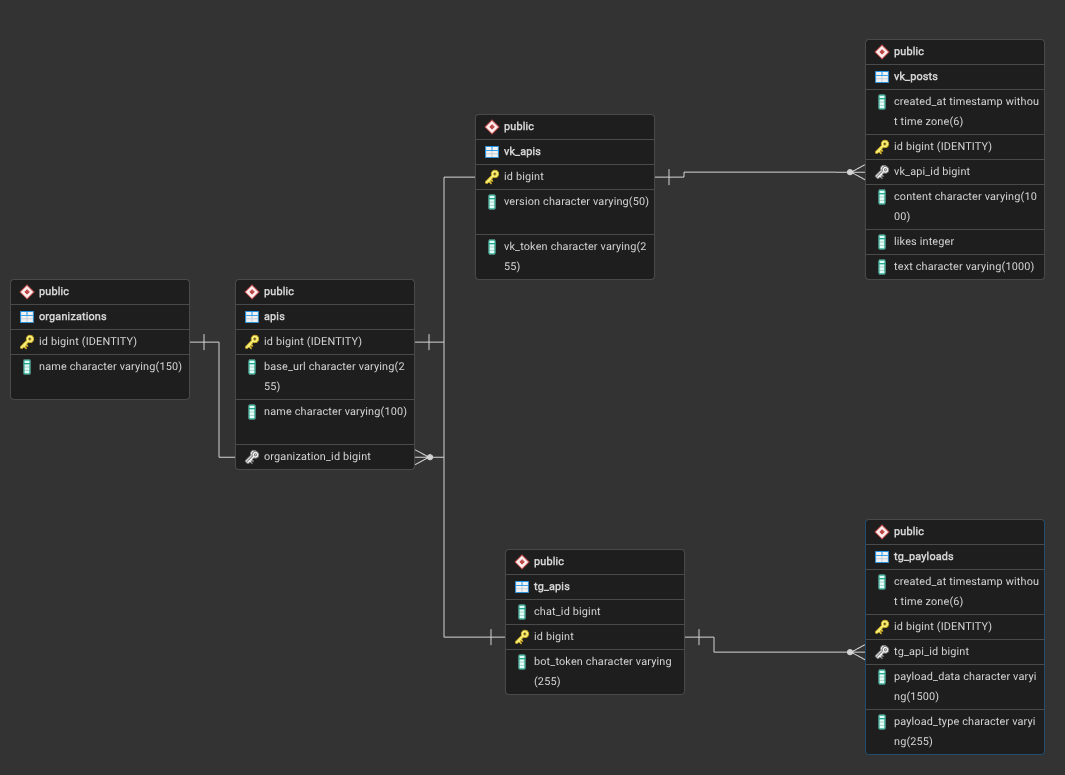
\includegraphics[width=\textwidth]{1.png}
    \caption*{Рисунок \arabic{imgcnt} -- ERD диаграмма}
    \stepcounter{imgcnt}
\end{figure}


\newpage
\clearpage

\section*{\normalsize Диаграмма классов}
\begin{figure}[!h]
    \centering
    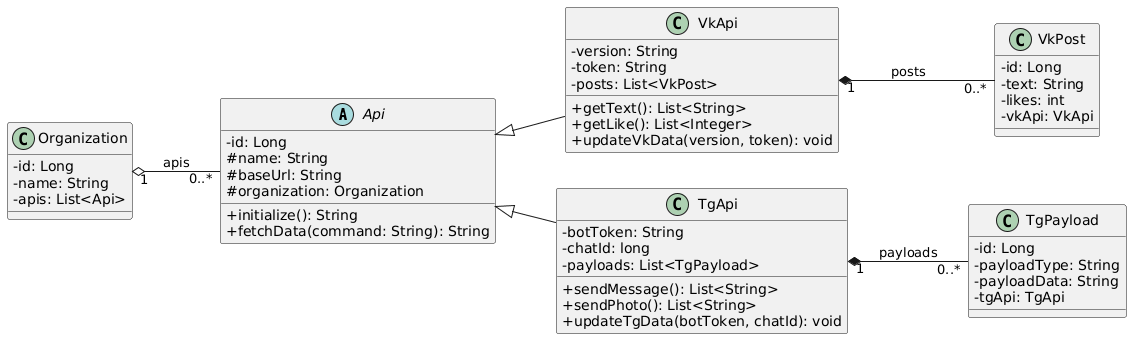
\includegraphics[width=\textwidth]{2.png}
    \caption*{Рисунок \arabic{imgcnt} -- Диаграмма классов}
    \stepcounter{imgcnt}
\end{figure}

\newpage
\clearpage



\section*{\normalsize Вывод}

Цель лабораторной работы достигнута, а задание выполнено полностью: разработано web-приложение на Java для предметной области VK и Telegram API с хранением данных в PostgreSQL и работой через Hibernate/JPA. CRUD-операции реализованы через \texttt{CrudRepository/JpaRepository}, а структура БД включает связанные таблицы и связи не только по наследованию.\

В процессе выполнения работы я научилась описывать модель предметной области через JPA-аннотации, настраивать наследование сущностей (\texttt{JOINED}), строить связи \texttt{one-to-many/many-to-one}, работать с сервисным и контроллерным слоями Spring Boot и вызывать методы предметной области через HTTP API.\

Основные сложности возникли при работе с Hibernate: корректная настройка связей между сущностями, требования к конструкторам по умолчанию, а также понимание того, как JPA автоматически формирует таблицы и внешние ключи. После настройки аннотаций и проверки схемы в PostgreSQL эти проблемы были решены.

\end{document}
